\documentclass[12pt,a4paper]{article}

% Packages
\usepackage[utf8]{inputenc}
\usepackage[T1]{fontenc}
\usepackage{graphicx}
\usepackage{amsmath}
\usepackage{amssymb}
\usepackage{hyperref}
\usepackage{geometry}
\geometry{margin=1in}

% Title and author information
\title{IMMUN4CARE WP1-3\\Mathematical Models for Immunology}
\author{IHU IMMUN4CARE Research Team}
\date{\today}

\begin{document}

\maketitle

\begin{abstract}
This document presents mathematical models and analysis for the IMMUN4CARE project, Work Package 1-3. The project focuses on immunological research and the development of mathematical frameworks to understand immune system dynamics.
\end{abstract}

\section{Introduction}

The IMMUN4CARE project aims to advance our understanding of immune system dynamics through mathematical modeling and computational approaches. This work package (WP1-3) focuses on developing and validating mathematical models that capture key immunological processes.

\section{Mathematical Framework}

\subsection{Basic Immune Response Model}

A fundamental model of immune response can be described by the following system of differential equations:

\begin{equation}
\frac{dP}{dt} = r P \left(1 - \frac{P}{K}\right) - \delta P I
\end{equation}

\begin{equation}
\frac{dI}{dt} = s P I - \mu I
\end{equation}

where:
\begin{itemize}
    \item $P$ represents the pathogen population
    \item $I$ represents the immune cell population
    \item $r$ is the pathogen growth rate
    \item $K$ is the carrying capacity
    \item $\delta$ is the pathogen clearance rate
    \item $s$ is the immune cell stimulation rate
    \item $\mu$ is the immune cell decay rate
\end{itemize}

\subsection{Model Analysis}

The equilibrium points of the system can be found by setting both derivatives to zero. This yields important insights into the long-term behavior of the immune response.

\section{Results}

\subsection{Numerical Simulations}

Figure~\ref{fig:immune_response} shows a typical immune response trajectory over time.

\begin{figure}[h]
\centering
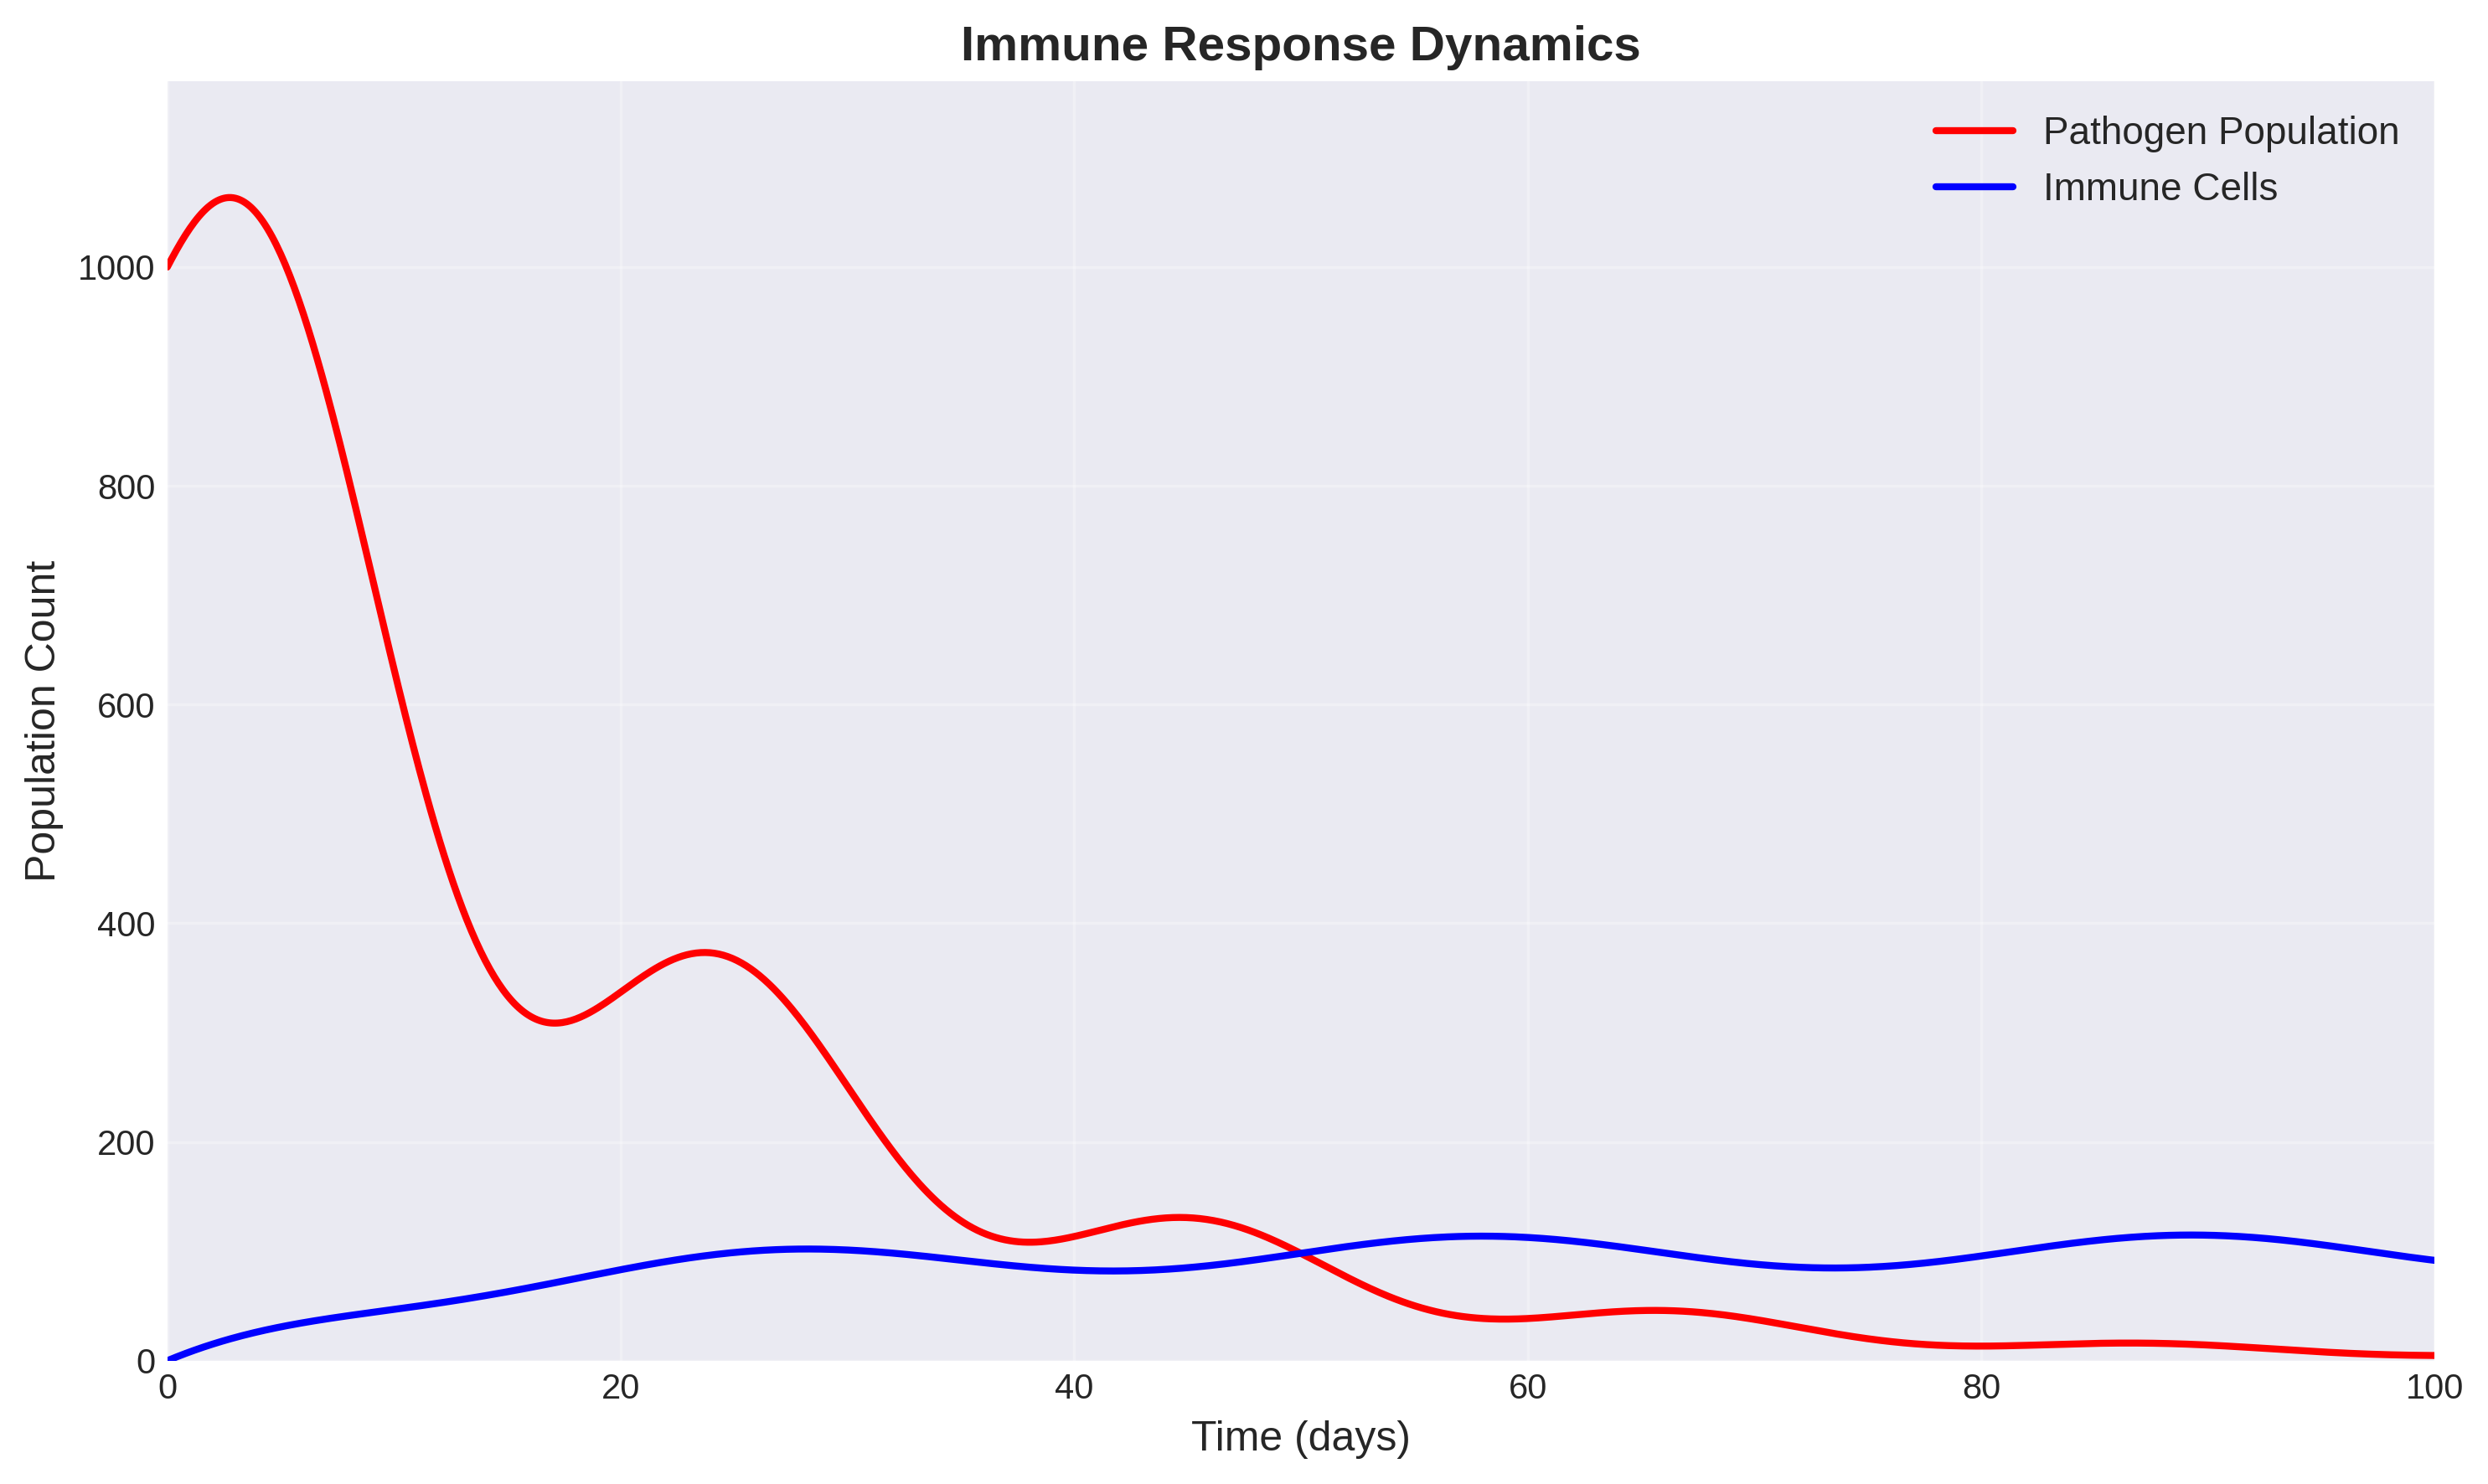
\includegraphics[width=0.7\textwidth]{figures/immune_response.png}
\caption{Time course of immune response showing pathogen and immune cell populations.}
\label{fig:immune_response}
\end{figure}

\subsection{Parameter Sensitivity}

Understanding how model parameters affect outcomes is crucial. Figure~\ref{fig:sensitivity} illustrates the sensitivity of the model to key parameters.

\begin{figure}[h]
\centering
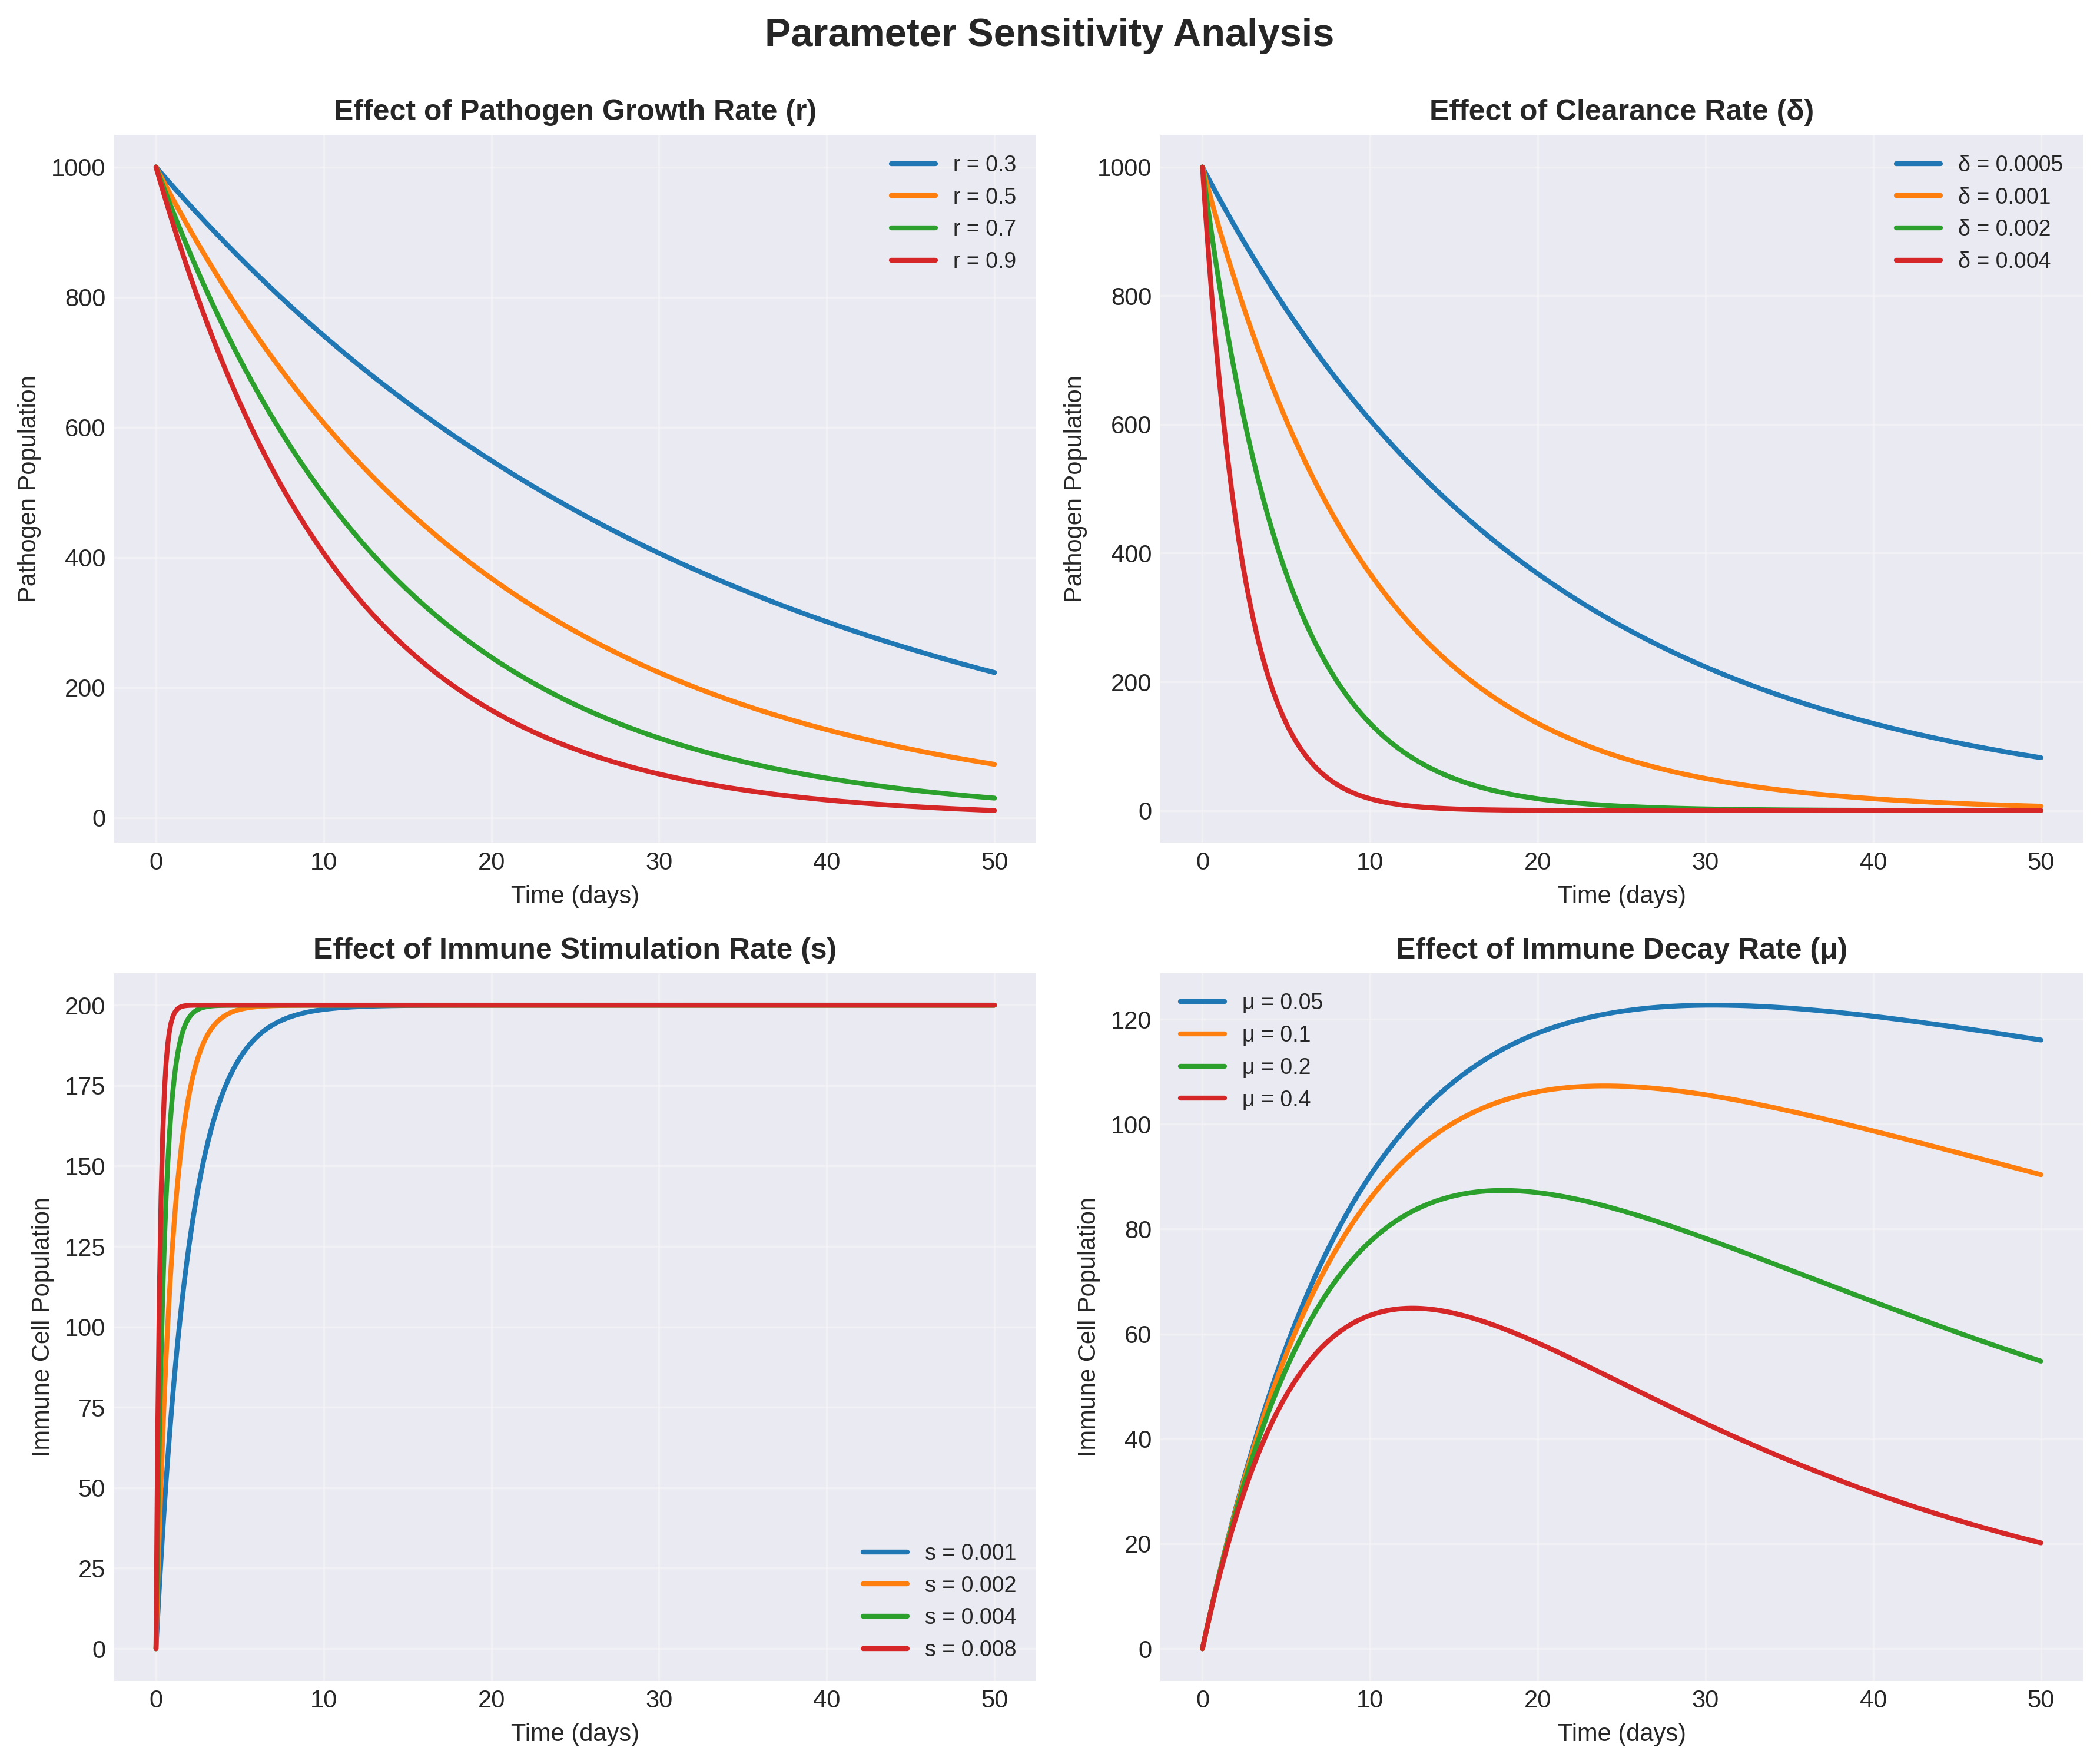
\includegraphics[width=0.7\textwidth]{figures/parameter_sensitivity.png}
\caption{Parameter sensitivity analysis showing the impact of varying key model parameters.}
\label{fig:sensitivity}
\end{figure}

\section{Discussion}

The mathematical models presented here provide a framework for understanding immune system dynamics. These models can be extended to incorporate additional biological details such as:

\begin{itemize}
    \item Multiple immune cell types
    \item Spatial dynamics
    \item Stochastic effects
    \item Treatment interventions
\end{itemize}

\section{Conclusions}

This work establishes a foundation for mathematical modeling of immunological processes within the IMMUN4CARE project. Future work will focus on parameter estimation from experimental data and model validation.

\section*{Acknowledgments}

This work is part of the IHU IMMUN4CARE project WP1-3. We acknowledge the support of all project partners and collaborators.

\bibliographystyle{plain}
% \bibliography{references}  % Uncomment when references.bib is created

\end{document}
